% This is a general template file for the LaTeX package SVJour3
% for Springer journals. Original by Springer Heidelberg, 2010/09/16
%
% Use it as the basis for your article. Delete % signs as needed.
%
% This template includes a few options for different layouts and
% content for various journals. Please consult a previous issue of
% your journal as needed.
%
\RequirePackage{fix-cm}
\RequirePackage{amsmath}  % for \text in math formulas: 
\RequirePackage[final]{graphicx}


%
%\documentclass{svjour3}                     % onecolumn (standard format)
%\documentclass[smallcondensed]{svjour3}     % onecolumn (ditto)
%\documentclass[smallextended]{svjour3}      % onecolumn (second format)
\documentclass[twocolumn]{svjour3}           % twocolumn 
% https://www.overleaf.com/23677550mgmxmmkvyxhf
%
\smartqed  % flush right qed marks, e.g. at end of proof


\usepackage[T1]{fontenc}
%\usepackage[utf8]{inputenc}

\usepackage{csquotes}
\usepackage{hyperref} % \url
\usepackage{gensymb}  % \degree
\usepackage{multirow}
\usepackage{xr}       % cross-references to supplementary
\usepackage{float}
\usepackage{xfrac}
\usepackage[dvipsnames]{xcolor}
%\usepackage{array}
%\usepackage{hhline}
%\usepackage{makecell}

%\renewcommand\cellgape{\Gape[6pt]}
%\renewcommand\theadfont{\itshape}

% special stuff for xr package, copied from here: 
% https://www.overleaf.com/learn/how-to/Cross_referencing_with_the_xr_package_in_Overleaf
\makeatletter
\newcommand*{\addFileDependency}[1]{% argument=file name and extension
  \typeout{(#1)}
  \@addtofilelist{#1}
  \IfFileExists{#1}{}{\typeout{No file #1.}}
}
\makeatother
\newcommand*{\supplementary}[1]{%
    \externaldocument{#1}%
    \addFileDependency{#1.tex}%
    \addFileDependency{#1.aux}%
}
\newcommand*{\maintext}[1]{%
    \externaldocument{#1}%
    \addFileDependency{#1.tex}%
    \addFileDependency{#1.aux}%
}
% end of stuff for xf/supplementary

\newcommand{\SVETE}{\color{Brown}}
%\newcommand{\SVETE}{{}}

%\newcommand{\ORANGE}[1]{\colorbox{BurntOrange}{#1}}

\newcommand{\tabhline}{\noalign{\smallskip}\hline\noalign{\smallskip}}

\newcommand*{\gtwoXY}[2]{\ensuremath{\Gamma_\text{2{#2}}^\text{#1}}}
\newcommand*{\gtwoY}[1]{\ensuremath{\Gamma_\text{2{#1}}}}
\newcommand{\Hfirst}{\ensuremath{\text{H}}}
\newcommand{\Hprime}{\ensuremath{\text{H}'}}
\newcommand{\Hone}{\ensuremath{\text{H}^1}}
\newcommand{\Htwo}{\ensuremath{\text{H}^2}}
\newcommand{\gtwo}{\ensuremath{\Gamma_2}}
\newcommand{\gtwoCSA}{\ensuremath{\Gamma_2^c}}
\newcommand{\gtwoXH}{\ensuremath{\Gamma_{\text{2XH,XH}'}}}
\newcommand{\gtwoCH}{\ensuremath{\Gamma_{\text{2CH,CH}'}}}
\newcommand{\gtwoNH}{\ensuremath{\Gamma_{\text{2NH,NH}'}}}
\newcommand{\gtwoXHa}{\ensuremath{\Gamma_\text{2XH,XH}}}
\newcommand{\gtwoCHa}{\ensuremath{\Gamma_\text{2CH,CH}}}
\newcommand{\gtwoNHa}{\ensuremath{\Gamma_\text{2NH,NH}}}
\newcommand{\gtwoNNH}{\ensuremath{\Gamma_\text{2N,NH}}}
\newcommand{\gtwoCCH}{\ensuremath{\Gamma_\text{2C,CH}}}
\newcommand{\gtwoXXH}{\ensuremath{\Gamma_\text{2X,XH}}}
\newcommand{\gtwoNNHp}{\ensuremath{\Gamma_{\text{2N,NH}'}}}
\newcommand{\gtwoCCHp}{\ensuremath{\Gamma_{\text{2C,CH}'}}}
\newcommand{\gtwoXXHp}{\ensuremath{\Gamma_{\text{2X,XH}'}}}

\newcommand{\StwoCH}{\ensuremath{S^2_\text{CH}}}
\newcommand{\StwoNH}{\ensuremath{S^2_\text{NH}}}
\newcommand{\StwoXH}{\ensuremath{S^2_\text{XH}}}
\newcommand{\StwoCHp}{\ensuremath{S^2_{\text{CH,CH}'}}}
\newcommand{\StwoNHp}{\ensuremath{S^2_{\text{NH,NH}'}}}
\newcommand{\StwoXHp}{\ensuremath{S^2_{\text{XH,XH}'}}}
\newcommand{\StwoCCH}{\ensuremath{S^2_\text{C,CH}}}
\newcommand{\StwoNNH}{\ensuremath{S^2_\text{C,NH}}}
\newcommand{\StwoXXH}{\ensuremath{S^2_\text{X,XH}}}

\newcommand{\JCH}{\ensuremath{J_{\text{CH,CH}'}}}
\newcommand{\JNH}{\ensuremath{J_{\text{NH,NH}'}}}
\newcommand{\JXH}{\ensuremath{J_{\text{XH,XH}'}}}
\newcommand{\JCCH}{\ensuremath{J_{\text{C,CH}}}}
\newcommand{\JNNH}{\ensuremath{J_{\text{N,NH}}}}
\newcommand{\JXXH}{\ensuremath{J_{\text{X,XH}}}}
\newcommand{\JHH}{\ensuremath{J_\text{HH}}}
\newcommand{\Jx}{\ensuremath{J_{\text{X}}}}
\newcommand{\Jxh}{\ensuremath{J_{\text{XH}}}}

\newcommand{\nclab}{\ensuremath{{}^{13}\text{C}/{}^{15}\text{N}}}
\newcommand{\nlab}{\ensuremath{{}^{15}\text{N}}}
\newcommand{\clab}{\ensuremath{{}^{13}\text{C}}}
\newcommand{\cnolab}{\ensuremath{{}^{12}\text{C}}}
\newcommand{\hlab}{\ensuremath{{}^{1}\text{H}}}
\newcommand{\dlab}{\ensuremath{{}^{2}\text{H}}}

\newcommand{\XHtwo}{\ensuremath{\text{XH}_2}}
\newcommand{\NHtwo}{\ensuremath{\text{NH}_2}}
\newcommand{\CHtwo}{\ensuremath{\text{CH}_2}}
\newcommand{\labNHtwo}{\ensuremath{{}^{15}\text{NH}_2}}
\newcommand{\labCHtwo}{\ensuremath{{}^{13}\text{CH}_2}}
\newcommand{\CHthree}{\ensuremath{\text{CH}_3}}

\newcommand{\sigmaIS}{\ensuremath{\sigma_{\text{IS}}}}
\newcommand{\qinner}{\enquote{inner}}
\newcommand{\qouter}{\enquote{outer}}

\newcommand{\oneJch}{\ensuremath{^1\!J_\text{CH}}}
\newcommand{\oneJnh}{\ensuremath{^1\!J_\text{NH}}}
\newcommand{\oneJxh}{\ensuremath{^1\!J_\text{XH}}}
\newcommand{\oneJcc}{\ensuremath{^1\!J_{\text{CC}}}}

\newcommand{\M}{\ensuremath{\hphantom{-}}}

\newcommand{\Iinn}{\ensuremath{I_\textrm{inn}}}
\newcommand{\Iout}{\ensuremath{I_\textrm{out}}}
\newcommand{\Ioutone}{\ensuremath{I_\textrm{out1}}}
\newcommand{\Iouttwo}{\ensuremath{I_\textrm{out2}}}

\newcommand*{\Xaa}[1]{\ensuremath{\textrm{\ensuremath{#1}}^{\alpha\alpha}}}
\newcommand*{\Xab}[1]{\ensuremath{\textrm{\ensuremath{#1}}^{\alpha\beta}}}
\newcommand*{\Xba}[1]{\ensuremath{\textrm{\ensuremath{#1}}^{\beta\alpha}}}
\newcommand*{\Xabba}[1]{\ensuremath{\textrm{\ensuremath{#1}}^{\alpha\beta + \beta\alpha}}}
\newcommand*{\Xabbam}[1]{\ensuremath{\textrm{\ensuremath{#1}}^{\alpha\beta - \beta\alpha}}}
\newcommand*{\Xbb}[1]{\ensuremath{\textrm{\ensuremath{#1}}^{\beta\beta}}}

% C±(HαHβ + HβHα) 
\newcommand{\TermInner}{\ensuremath{ 
  C_\pm (
     H_\alpha H'_\beta + 
     H_\beta H'_\alpha ) }}
% C±HαHα 
\newcommand{\TermOuterA}{\ensuremath{
  C_\pm H_\alpha H'_\alpha
}}
% C±HβHβ
\newcommand{\TermOuterB}{\ensuremath{
  C_\pm H_\beta H'_\beta
}}
%C±(HαHα + C±HβHβ) 
\newcommand{\TermOuter}{\ensuremath{ 
  C_\pm (
     H_\alpha H'_\alpha + 
     H_\beta H'_\beta ) }}
  



\supplementary{G2_Supplement}

% Insert the name of "your journal" with
\journalname{Journal of Biomolecular NMR}
%


\begin{document}

\title{Accurate measurement of dipole\slash dipole transverse 
  cross-correlated relaxation \gtwo{} in methylenes and primary 
  amines of uniformly \nclab-labeled proteins
}

%\subtitle{Do you have a subtitle?\\ If so, write it here}

% Grants or other notes about the article that should go on the front
% page should be placed within the \thanks{} command in the title
% (and the %-sign in front of \thanks{} should be deleted)
%
% General acknowledgments should be placed at the end of the article.



\titlerunning{Accurate measurement of \gtwo}       
\authorrunning{Lesovoy D.M. et. al.} % if too long for running head

\author{Dmitry M. Lesovoy 
        \thanks{corresponding author, e-mail:  lesovoydm@gmail.com} \and
        Maxim A. Dubinnyi      \and 
        Svetlana B. Nolde      \and 
        Eduard V. Bocharov  
          \thanks{corresponding author, e-mail:  bon@nmr.ru}\and 
        Alexander S. Arseniev
}



\institute{
  Dmitry M. Lesovoy    \and 
  Maxim A. Dubinnyi    \and 
  Svetlana B. Nolde    \and 
  Eduard V. Bocharov   \and 
  Alexander S. Arseniev
  \at
  Shemyakin{-}Ovchinnikov Institute of Bioorganic Chemistry, 
  Russian Academy of Sciences RAS,  Str. {Miklukho{‐-}Maklaya} 
  16/10, Moscow, 117997, Russian Federation 
\and
  Maxim A. Dubinnyi    \and 
  Eduard V. Bocharov   \and 
  Alexander S. Arseniev \at
  Moscow Institute of Physics and Technology (State University), 
  Institutsky per., 9, Dolgoprudny, 141700, Russian Federation  
}

\date{Received: date / Accepted: date}
% The correct dates will be entered by the editor

\maketitle

\begin{abstract}
Side chains possess a broader conformational space (compared to the 
backbone) and are directly affected by intra- and intermolecular 
interactions, hence their dynamics and the corresponding NMR relaxation 
data are more sensitive and informative. Nevertheless, transverse 
relaxation in \XHtwo{} ($\text{X}=\clab$ or \nlab) spin systems is 
predominantly non-measurable in uniformly \nclab-labeled 
proteins due to cross-correlation effects. In the present publication, we 
propose a number of pulse sequences for accurate and precise measurement 
of the dipole-dipole transverse cross-correlated relaxation rate 
\gtwoXH, which, similarly to $R_2$ measurements, 
provides information about the amplitudes of intramolecular dynamics. 
The suggested approach has allowed us to circumvent a number of obstacles 
that were limiting earlier applications of \gtwoXH: 
1) impossibility of transmission of the central component of the triplet 
of \XHtwo{} group to \hlab-acquisition via INEPT has been solved by 
transmission of the averaged signal of \qinner{} and \qouter{} 
components of the triplet; 
2) direct recording of the entire triplets resulting in substantial 
overlap of side chain signals has been replaced by recording of 
individual singlets with the use of \oneJch-modulated approach 
and constant-time evolution; 
3) low sensitivity has been enhanced via proton acquisition which 
required special attention to a zero-quantum coherence evolution. 
The proposed 
method expands the set of \enquote{dynamics sensors} covering protein side chains 
and substantially improves the quality and the level of detail of 
experimental data describing dynamic processes in proteins and protein 
complexes. 

\keywords{proteins \and NMR \and side chain dynamics \and methylenes  \and 
primary amines \and relaxation \and 
dipole/dipole transverse cross-correlated relaxation 
}
% \PACS{PACS code1 \and PACS code2 \and more}
% \subclass{MSC code1 \and MSC code2 \and more}
\end{abstract}

\section{Introduction}
\label{intro}

Measurement of relaxation parameters of nuclear spins and superposition
of various multispin density operators provides unique information about mobility
of different groups of protein atoms. However, due to the complexity of
NMR relaxation mechanisms, many of the parameters of the relaxation 
matrix cannot be practically measured; therefore only some of them 
found broad application in routine protein studies. For example, 
relaxation parameters of backbone NH groups: \nlab{} longitudinal 
($R_1$) and transverse ($R_2$) relaxation rates, heteronuclear 
$\nlab-\{\hlab\}$ NOE (\sigmaIS), and dipole\slash CSA transverse 
cross-correlated relaxation \gtwoNNH, are in the mainstream 
\cite{ishima_recent_2011,palmer_1.13_2012}.
Other components of the NH group relaxation matrix (e.g., the rates of
\hlab{} longitudinal and transverse relaxation) cannot be measured. 
However, the interpretation of the four experimentally accessible 
relaxation parameters of an NH group ($R_1$, $R_2$, \sigmaIS{} 
and \gtwoNNH) yields a holistic picture of its dynamics: 
the order parameter $S^2$, the overall and the internal rotational 
correlation times ($\tau_c$ and $\tau_e$), and the identification of 
exchange processes. 

In comparison with the backbone NH groups, mobility of the protein side 
chains is a more attractive sensor for investigation of protein dynamics, 
since the protein side chains have a broader conformational space and are 
directly susceptible to the effects of protein interactions 
\cite{igumenova_characterization_2006,paquin_multiple-timescale_2008,trbovic_protein_2009,yang_probing_2011,weininger_13c_2012,ferrage_chapter_2017}. 
Thus, it is the side chain mobility 
monitoring that provides a better understanding of binding the 
protein surface with a partner, which is especially important 
for understanding the function of protein hot-spots at the atomic level 
\cite{zerbe_relationship_2012,cukuroglu_hot_2014,watkins_side-chain_2016}. 
Nevertheless, measurements of side chain NMR-relaxation parameters are used 
much less frequently due to numerous complications of both technical and 
fundamental nature. In order to investigate the mobility of side chains, 
researchers have to choose between two strategies: either apply 
sophisticated and costly methods of selective labelling or use simple and 
readily available methods of uniform \nclab{} labelling. In the 
first case, partial deuteration and alternating \clab--\cnolab{} labelling 
patterns used for \dlab{} relaxation studies or \nclab{} relaxation 
measurements \cite{kushlan_proton-detected_1993,lemaster_dynamical_1996} 
in $^{13}\text{CHD}$, $^{15}\text{NHD}$, and $^{13}\text{CHD}_2$ 
groups remarkably simplify \cite{lemaster_nmr_1999} relaxation studies 
but are associated with the confounding effects of isotope scrambling. 
In the latter case, experimentally available data are limited to only 
two credibly measurable 
\nclab{} relaxation parameters: $R_1$ and NOE 
\cite{yang_probing_2011,ferrage_chapter_2017}, 
and these parameters do not provide a detailed vision of the 
dynamic processes, in which an \XHtwo{} group is involved. As far as 
$R_2$ is concerned, a number of difficulties arise: for example, the 
carbon-carbon \oneJcc{} interaction during {CPMG}, as well as 
cross-correlation effects, though considered as negligible in some pioneering works 
\cite{buck_structural_1995}. However, in more recent articles it 
has been recognised that these effects may result in problematic 
measurements and analysis and cannot be eliminated by an 
appropriate design of the pulse sequence
\cite{yang_probing_2011,kumar_cross-correlations_2000}.

In uniformly labelled proteins, an alternative to $R_2$ is the transverse 
cross-correlated relaxation rate \gtwoXH, which, similarly to $R_2$, 
provides information about the spectral density function at zero frequency 
$J(0)$ and hence characterizes amplitudes of intramolecular dynamics 
\cite{yang_probing_2011}. The measurement and analysis of the 
di\-pole\slash{} CSA transverse cross-correlated relaxation \gtwoNNH{} 
have become a classical tool for backbone NH groups in solution {NMR}, 
since it readily provides the parameters of local motions $\tau_r$ 
\cite{chill_measurement_2006} and, in combination with other relaxation 
parameters, can give a detailed picture of internal dynamics 
\cite{cavanagh_protein_2007,charlier_protein_2016}. As for the \CHthree{} 
groups, the measurement of \gtwoCH{} in uniformly \nclab-labeled proteins 
is based on the analysis of \qinner\slash \qouter{} intensity ratio in 
\clab{} quadruplets \cite{zhang_probing_2006} and allows, for example, 
mapping the interfaces of helix-helix interactions in membrane proteins 
\cite{lesovoy_nmr_2017}. In order to comprehensively describe how the 
protein surface dynamically adapts to interaction with a binding 
partner, monitoring of \CHtwo{} and \NHtwo{} groups is also needed. 
Unfortunately, for \CHtwo{} and \NHtwo{} groups the analysis of 
intensities in the conventional constant-time {HSQC}-type \hlab-detected 
experiments \cite{zhang_probing_2006,lesovoy_nmr_2017} provides no 
information about the ratio of intensities of \qinner{} and \qouter{}
components in \CHtwo{} triplet, since the \qinner{} component 
\TermInner{}
does not evolve under \oneJch{} scalar coupling Hamiltonian, 
and hence it cannot be transferred to \hlab-acquisition with the aid 
of back {INEPT}. In addition to 1D carbon-detected experiments, that 
do not provide adequate resolution for proteins 
\cite{ghalebani_nmr_2008,kaderavek_spectral_2016}, 2D experiments with
indirect detection of \clab{} triplets and transfer of coherence to
$(\text{C}_\alpha) \text{H}_\alpha$ have been suggested for methylenes 
\cite{banci_side_2001}, but detect only some $\text{C}_\beta$ due to 
signal overlapping and artifacts of water suppression. 3D experiments 
based on the indirect detection of \clab{} triplets via CC(CO)NH {TOCSY} or CBCA(CO)NH schemes have also been proposed \cite{zheng_measurement_2004,yang_1h13c_1999},
but have limited sensitivity, especially for the methylene groups 
remote from the backbone. 

In the present work, we suggest a number of experiments for measuring 
\gtwoXH{} in methylenes and primary amines, aimed at complementing the
methods proposed earlier for methyls 
\cite{zhang_probing_2006,lesovoy_nmr_2017}. 
In the search for an optimal approach, we tested three diverse pulse 
sequences: 
(i) 2D \hlab-\clab{} carbon-detected \oneJch-resolved experiment, 
which allows conventional recording of the change in the ratio of multiplet components, but has a relatively low sensitivity and leads to a considerable overlap between the signals (it may serve as a reference to the following experiments); 
(ii) 2D \hlab-\clab{} carbon-detected \oneJch-modulated experiment with 
no cross peak splitting due to \oneJch{} constant, which mostly resolves 
the issue of signal overlapping, but leaves the issue of sensitivity 
unsolved; and 
(iii) 2D proton-detected \oneJch-modulated experiment with a zero-quantum coherence converted to separate undetectable terms, 
which allows effectively measuring 
\gtwoXH{} at the most of side chain \XHtwo{} positions without any 
considerable loss of sensitivity and resolution. 
A small ($\tau_c \sim 3$ 
ns) 61-residue water-soluble protein neurotoxin II (NTII, well studied in the past 
in our laboratory 
\cite{lesovoy_specific_2009,bocharov_resonance_2003,krabben_loop_2009}
was chosen 
as a model system for pulse sequence development and appraisal. We provide an example of the simple analysis of relaxation parameters \gtwoCH{} obtained for methylenes of NTII.

\section{Theory: transverse relaxation in \XHtwo{} groups}
\label{sec:theory}


Relaxation processes of three coupled spin-$\sfrac{1}{2}$ nuclei in isolated 
\XHtwo{} group (X=\nlab{} or \clab{}) are driven by dipole-dipole (DD) and 
CSA\slash dipole (chemical shift ani\-so\-tro\-py) interactions of the X and 
two \hlab{} spins resulting in 
auto- and cross-relaxation rates reviewed elsewhere 
\cite{kumar_cross-correlations_2000,zheng_measurement_2004}. 
The interference of different relaxation mechanisms provides the basis for
\CHtwo-{TROSY} experiment \cite{miclet_relaxation-optimized_2004} which 
yields a considerable enhancement in resolution and sensitivity.

After \oneJxh-splitting by the directly 
attached protons the X nucleus undergoes differential relaxation of  
\Xaa{X}, \Xabba{X} and \Xbb{X} triplet components, where $\alpha$ and $\beta$
refers to $|\alpha\rangle$ and $|\beta\rangle$ spin states of the two coupled
protons \Hfirst{} and \Hprime{}.
Although the most general description of transverse relaxation deals with $4\times 4$ 
relaxation matrix in irreducible basis representation 
\cite{kay_heteronuclear_1992,prestegard_characterization_1978},
distinct transverse relaxation rates of individual components proved
to be effective \cite{zheng_measurement_2004} for proteins with the 
overall rotational correlation time $\tau_c < 9$~ns during the typical 
constant-time relaxation delay $1/\oneJcc = 28.6$ ms.

Individual transverse relaxation rates of the triplet components are 
\cite{kumar_cross-correlations_2000,banci_side_2001,miclet_relaxation-optimized_2004}:
\begin{subequations}
\label{eq:grates} 
\begin{align}
\label{eq:gaa} 
  \Xaa{\Gamma}    & = \Gamma_2^a + \gtwo + 2 \gtwoCSA  \\
  \label{eq:gab} 
  \Xabba{\Gamma}  & = \Gamma_2^a - \gtwo \\
  \label{eq:gbb} 
  \Xbb{\Gamma}    & = \Gamma_2^a + \gtwo - 2 \gtwoCSA
\end{align}
\end{subequations}
where $\Gamma_2^a$ represents all relaxation rates with equal contribution 
to all  multiplet components, \gtwo{} is the dipole\slash dipole transverse 
cross-correlated relaxation rate (the rate of interest) and \gtwoCSA{} is 
the CSA\slash dipole transverse cross-correla\-ted relaxation:
\begin{subequations}
\label{eq:gcompounds} 
\begin{align}
 \label{eq:g2a} 
 \Gamma_2^a & = \gtwoXY{}{X\Hfirst,X\Hfirst} + 
               \gtwoXY{}{X\Hprime,X\Hprime} +
               \gtwoXY{}{X,X} + \cdots \\
 \label{eq:g2} 
 \gtwo & \equiv \gtwoXY{}{X\Hfirst,X\Hprime} \\
  \label{eq:g2c} 
 \gtwoCSA & \equiv \gtwoXY{}{X,X\Hfirst} 
\end{align}
\end{subequations}
Terms in (\ref{eq:g2},~\ref{eq:g2c}) are responsible for
differential relaxation rates of multiplet components.
During the relaxation delay $T$ intensities of three
mul\-ti\-plet components decay exponentially 
with rates \eqref{eq:grates} to
\begin{subequations}
\label{eq:gintensity} 
\begin{align}
  \label{eq:gint:aa} 
    \Xaa{I}(T)    = \Ioutone & = I(0)\exp(-\Xaa{\Gamma} T) \\
  \label{eq:gint:abba} 
    \Xabba{I}(T)  = \Iinn  &  = 2 I(0)\exp(-\Xabba{\Gamma} T) \\
  \label{eq:gint:bb} 
  \Xbb{I}(T)   = \Iouttwo &= I(0)\exp(-\Xbb{\Gamma} T) 
\end{align}
\end{subequations}

The values of \gtwo{} and $\Gamma_2^c$ can be calculated from the intensities 
of individual lines by combination of 
\eqref{eq:grates} and \eqref{eq:gintensity}:
\begin{align}
\label{eq:gtwofromint}
  \gtwo & = - \frac{1}{4T} ln\biggl(\frac{4 \Ioutone \Iouttwo}{\Iinn^2}\biggr)\\
\label{eq:gcsafromint}
  \gtwoCSA & = - \frac{1}{4T} ln\biggl(\frac{\Ioutone}{\Iouttwo}\biggr)
\end{align}
Equation \eqref{eq:gtwofromint} is the method of consensus for the measurement of 
\gtwo{}
\cite{banci_side_2001,zheng_measurement_2004,yang_study_1998}. 

The dipole\slash dipole \gtwo{} \eqref{eq:g2} and the 
CSA\slash dipole \gtwoCSA{} \eqref{eq:g2c} transverse 
cross-correlated relaxation rates are governed by the dynamics of an 
\XHtwo{} group as follows 
\cite{yang_probing_2011,kumar_cross-correlations_2000,banci_side_2001,zheng_measurement_2004,yang_study_1998}:
\begin{align}
  \label{eq:gtwoJ}
  \gtwo  & = 
    \tfrac{1}{10} \xi_\text{XH}^2
       \Bigl(4 \Jxh(0) + 3 \Jxh(\omega_\text{X} ) \Bigr )  \\
  \label{eq:gtwoCSAJ}
  \gtwoCSA & = \tfrac{1}{15} \xi_\text{X} \xi_\text{XH}
    \Bigl(4 \Jx(0) + 3 \Jx(\omega_\text{X} ) \Bigr )
\end{align}
where scaling constants for the dipole\slash dipole and the CSA\slash 
dipole interactions are:
\begin{align}
  \xi_\text{XH} = &  
     \frac{\mu_0 \hbar \gamma_H \gamma_X }{4 \pi r_\text{XH}^3 }, 
  \thickspace\thickspace 
      \xi_\text{X} = \omega_\text{X} \Delta \sigma_\text{X} \\
  \Delta\sigma_\text{X} = & \sigma_x P_2(\cos x)+\nonumber \\
  & \sigma_y P_2(\cos y) + \sigma_z P_2(\cos z)
\end{align}
Spectral density functions in the model-free approximation of Lipari and Szabo 
\cite{lipari_model-free_1982} with an isotropic 
overall rotation are:
\begin{align}
  \label{eq:Jxh}
    \Jxh(\omega)  = & \StwoXHp\frac{ \tau_c}{1 + (\omega \tau_c)^2} 
     + \nonumber \\
     + & \bigl[ P_2(\cos\theta_\text{{HXH}'})-\StwoXHp\bigr]
     \frac{\tau_e}{1+(\omega\tau_e)^2}\\
  \label{eq:Jx}
    \Jx(\omega)  = & \StwoXXH \frac{\tau_c}{1 + (\omega \tau_c)^2} 
    + \nonumber \\
    + & \bigl[ P_2(\cos\theta_\text{X})-\StwoXXH\bigr]
     \frac{\tau_e}{1+(\omega\tau_e)^2}
\end{align}

In equations (\ref{eq:gtwoJ}--\ref{eq:Jx}) $\text{X} =\clab$ or \nlab;
$\mu_0$ is the vacuum permeability; 
$\hbar$ is Planck's constant; 
$\gamma_H$, $\gamma_C$, $\gamma_N$ are the gyromagnetic ratios of
  \hlab{}, \clab{} and \nlab;
$\Delta\sigma_\text{X}$ is chemical shift anisotropy of spin X;
$\cos x$, $\cos y$, $\cos z$ are the direction 
  cosines of the XH bond vector in the principle frame
  of the CSA tensor of spin X;
$P_2(x) = \tfrac{1}{2}(3x^2-1)$;
$\omega_N$, $\omega_C$ are carbon and nitrogen Larmor frequencies;
$r_\text{XH}$ is the {CH} or {NH} distance, 
$r_\text{CH} = 1.09$~\AA{} and $r_\text{NH} = 1.00$~\AA;
$\tau_c$ and $\tau_e$ denote overall and local rotational 
  correlation times, respectively; 
\StwoXHp{} and \StwoXXH{} are the generalized cross-correlation 
  order parameters of dipole\slash dipole and CSA\slash 
  dipole interactions,respectively.

To complete the picture we should note that some minor 
relaxation terms including proton-proton interactions
were neglected here, but their overall contribution to \gtwo{} 
does not exceed $0.4\,s^{-1}$ 
\cite{zheng_measurement_2004}.

The term $J(0)$ is dominant in the equations \eqref{eq:gtwoJ} and 
\eqref{eq:gtwoCSAJ}.
Assuming fast internal dynamics in comparison with the overall rotational 
correlation time ($\tau_e \ll \tau_c$)  \gtwoCH{} is 
simplified to
\begin{align}
  \label{eq:gtwo:tauc}
  \gtwo  \approx \frac{1}{10}  \xi_\text{XH}^2
  \biggl(4 \tau_c + \frac{3 \tau_c}{1 + (\omega_X \tau_c )^2 } 
  \biggr ) \StwoXHp
\end{align}
Such an approximation has been tested earlier in the work of Zheng and Yang 
\cite{zheng_measurement_2004} and found to give the systematic error for 
\gtwoCH{} estimates less than $0.4 s^{-⁠1}$ under the following 
limiting conditions for correlation times: $0 < \tau_e \le 500$ ps and 
$3 < \tau_c \le 12$ ns.


\section{Materials and methods}
\label{mmeth}

NMR experiments were performed on an {AVANCE}-{III}-800 spectrometer 
(\enquote{Bruker}, Germany) equipped with 5mm {CPTCI} {1H-13C/15N/D} 
{Z-GRD} cryoprobe. A uniformly \nclab-labeled sample of 0.8 mM 
neurotoxin II, pH 5.0, 95\% $\text{H}_2\text{O}$, 5\% 
$\text{D}_2\text{O}$, 30\degree {C} at 50 mM 
ionic strength in a Shigemi tube was used. All experimental details 
concerning protein expression and purification were the same as in 
\cite{bocharov_resonance_2003}. NMR experiments used for signal 
assignment and structure determination are present in the protein 
data bank (structure set 2MJ4) and BMRB (data set 19704). Spectra 
acquisition, processing, and analysis were performed using TopSpin 
(\enquote{Bruker}, Germany) and CARA (\url{http://www.nmr.ch}) 
programs. \hlab-\clab{} 2D correlation carbon-detected experiments 
were recorded as a complex matrix of $256\times 2048$ data points 
with the spectral width of $4.5$ ppm and 100 ppm in the indirect 
\hlab{} and direct \clab{} dimensions, respectively. Constant-time 
{HSQC}-based proton-detected experiments were recorded with the 
spectral width of $32.2$ ppm (number of data points depends on a 
constant time period) in the indirect \clab{} dimension and 12 ppm 
(2048 data points) in the direct \hlab{} dimension. The number of 
scans for each point in the indirect dimension varies from 32 to 
256 rising with the transverse relaxation delay $T$. The recycle 
delay of $1.2$ s was applied for all experiments. 

The inversion pulse for \clab{} aliphatic region was a smoothed
linear Chirp of $500 \mu s$ duration, 60 kHz total sweep width, with 
offset at 36 ppm, defined by 1000 points, 20\% smoothing, sweep from 
high to low field (Crp60,0.5,20.1 in the Bruker wave form library)
\cite{kupce_optimized_1996,fu_broadband_1995}
calibrated with Q factor of 5. The inversion pulse for \hlab{} zero-quantum dephasing \cite{thrippleton_elimination_2003,harris_zero-quantum_2011} was a smoothed linear Chirp of 40 ms duration, 60 kHz total sweep width, with 
offset at 4.7 ppm, defined by 20000 points, 20\% smoothing, sweep from 
high to low field (Crp60,40,20.20 in the Bruker wave form library) calibrated with Q factor of 5. Water \hlab{} flip-back 90\degree{} pulses were a sinc-shaped \cite{cavanagh_protein_2007} (1000 points defining the shape) of 3 ms duration with offset at 4.7 ppm. Selective inversion of CO and aromatic carbons was done by the classical inversion shape pulse IBurp1 (1000 points defining the shape) of 265 $\mu s$ duration with offset at 145 ppm
\cite{geen_band-selective_1991,vincent_chapter_1997}.
 A carbon 180\degree{} Quaternion cascade (Q3) shaped pulse of 
 $220 \mu s$ duration (1000 points defining the shape) with offset at 
 36 ppm  \cite{vincent_chapter_1997,emsley_optimization_1992}
 was applied to invert and refocus the aliphatic region simultaneously
 without \oneJch{}-evolution \cite{lescop_guidelines_2010}
 during the pulse. It should be noted that shaped composite $\pi$ pulses
 such as CHIRP (Crp80comp.4) \cite{hwang_broadband_1997}
 or REBURP \cite{geen_band-selective_1991}
 cannot be used here for both inversion and refocusing \cite{xia_enhancing_2017}.

The values of \oneJxh{} scalar couplings in \XHtwo{} groups were 
found with the aid of \hlab-detected constant-time {HSQC}-based 
experiment \cite{zhang_probing_2006,lesovoy_nmr_2017}, which was 
designed initially for methyl groups and could not transfer the 
\qinner{} component of \clab{} triplet \TermInner{}
of a methylene group. Accordingly, only the \qouter{} \TermOuter{}
components were detected evolving as 
$\cos(2\pi \cdot {\oneJch} \cdot t)$, thus providing \oneJch{} 
values. Signal intensity analysis was performed with the aid of 
Mathematica (Wolfram Research Inc.). The program minimizes a penalty 
function (the difference between experimental and theoretical values) 
by the method of Levenberg-Marquardt \cite{press_chapter_1992} and 
yields estimates of the parameters together with their uncertainties. 
The details of the analysis contributed to \gtwoXH{} relaxation 
parameter estimates are step by step described in the Results. 
Isotropic rotational diffusion tensor with $\tau_c = 3$ ns was used to 
describe the overall tumbling of the protein for the interpretation 
(finding order parameters of internal motions) of side chain relaxation. 
Diffusion tensor parameters were determined by the aggregate analysis of 
all backbone \nlab{} relaxation parameters with the help of the 
FastModelFree software \cite{cole_fast-modelfree_2003}. The dependence 
of \gtwoCH{} upon the cross-correlation order parameter \StwoCHp{} was estimated 
by equation \eqref{eq:gtwo:tauc} for $\tau_c = 3$ ns and 
proton {NMR} frequency 800~MHz: 
\begin{align}
\label{eq:gapprox2}
     \StwoCHp  & \approx 0.037 \cdot \gtwoCH \\
     \StwoNHp  & \approx 0.130 \cdot \gtwoNH
\end{align}
Analysis of NMR pulse sequences with the product operator formalism was also performed in Mathematica (Wolfram Research Inc.) using "POMA" package \cite{guntert_poma:_1993,guntert_symbolic_2006,benesi_primer_2015}.


\section{Results}
\label{results}
Dipole-dipole transverse cross-correlated relaxation rate \gtwoXH{} mo\-dulate the \nclab{}
triplet intensities of a \CHtwo/\NHtwo{} group from the classic $1:2:1$ 
ratio towards a \enquote{distorted} one, where the intensity of the central 
component decrease and the sum of the side components increase during the 
relaxation delay \cite{yang_probing_2011,zheng_measurement_2004}. The 
easiest and the most obvious method of \gtwo{} measurement is to extract 
the ratio of the triplet components from a one-dimensional \clab{} 
experiment, which is practically unachievable due to a considerable overlap 
of the carbon signals of a typical protein. In order to measure \gtwo{} 
for proteins, we developed three pulse se\-quen\-ces, which sequentially solve 
and optimize the problem of quantification of the dipole-dipole transverse 
cross-cor\-related relaxation rate \gtwo.

\subsection{Scheme 1: \oneJch-resolved carbon-detected experiment}
\label{subseq:scheme1}

\begin{figure*}
 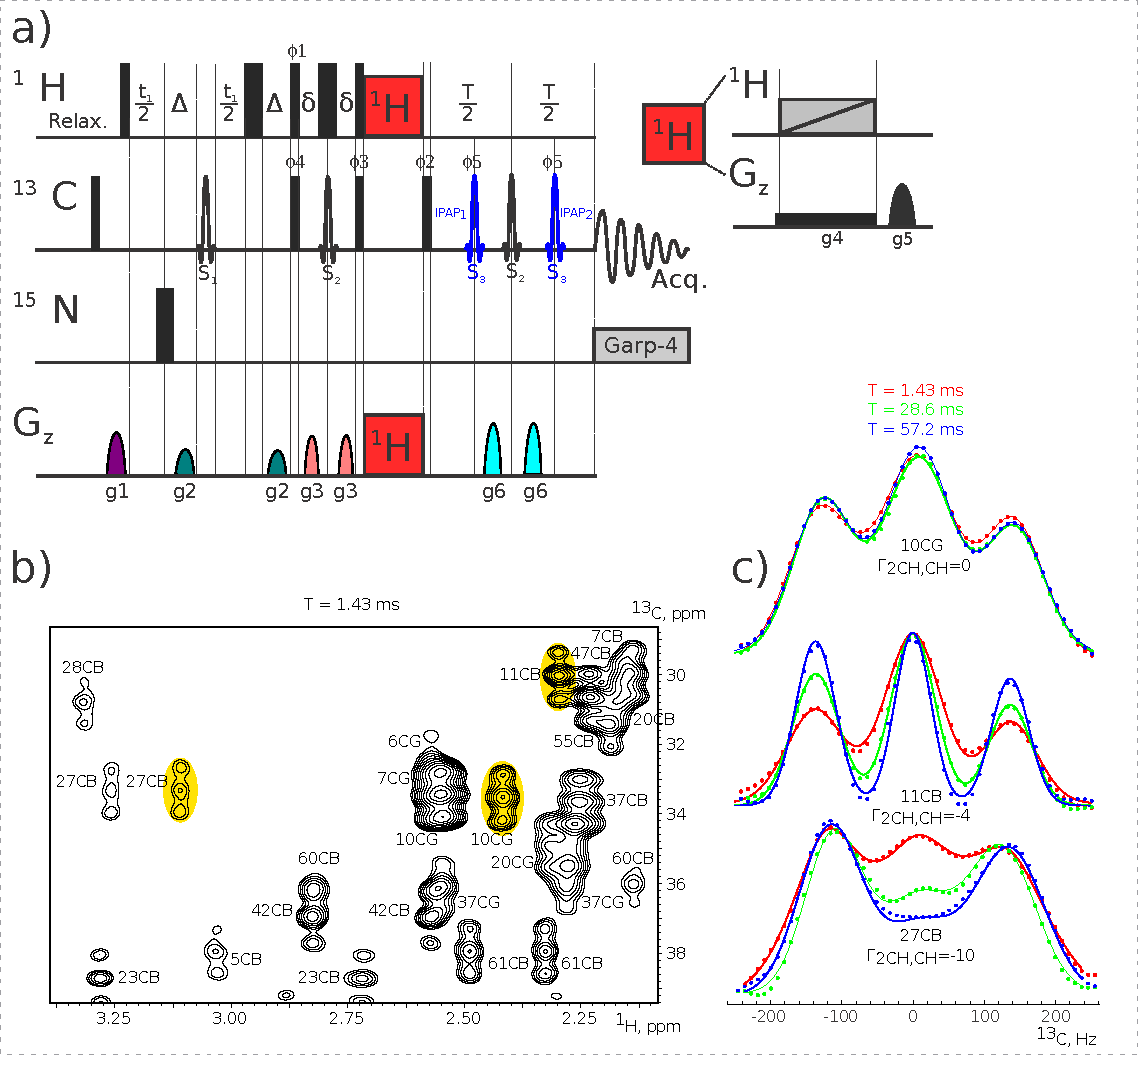
\includegraphics[width=1.0\textwidth]{Fig1}
 \caption{
 a) The pulse sequence of a 2D \hlab-\clab{} carbon-detected 
 \oneJch-resolved experiment (Scheme \ref{subseq:scheme1}) 
 to measure \gtwoCH{}. Narrow and thick bars represent 90\degree 
 and 180\degree pulses. Semi-constant-time \hlab{} States-{TPPI} 
 sampling is implemented with the aid of $t_1$ delay and 
 $\varphi_1$; {INEPT} delays are $\Delta = 2\delta = 1/(4\oneJch)$; 
 transverse relaxation delays $T$ are 1.43, 28.6 and 57.2 ms. 
 The red box represents a 42 ms block of \hlab{} inversion adiabatic pulse and gradients\cite{thrippleton_elimination_2003,harris_zero-quantum_2011}, suppressing all \hlab-containing coherences. 
 \nlab-decoupling is applied during acquisition. 
 S1 is a 500 $\mu s$ long \clab{} inversion adiabatic Chirp pulse. 
 S2 is a 220 $\mu s$ long 180\degree{} Q3 pulse (the offset at 36 ppm). 
 S3 (a 265 $\mu s$ long inversion IBurp1 pulse with the offset 
 at 145 ppm) is applied for virtual IPAP decoupling by simultaneous 
 altering the IPAP1 ($T/4$ or 4.5 ms) and IPAP2 ($T/4$ or 0 ms) 
 delays. Gradient pulses with squared sine shape and 1 ms length 
 except for g3 (0.6 ms), g4 (rectangular 40 ms) are used. 
 The g1-g7 gradient strengths are as follows: 27\%, 37\%, 47\%, 10\%, 35\%, and 57\%, whereas 100\% corresponds to 53.5 G/cm.
 The default phase is $x$ and the phase cycle is: 
 $\varphi_1 = y, -y$; 
 $\varphi_2 = 2(x), 2(-x)$; 
 $\varphi_3 = 4(x), 4(-x)$; 
 $\varphi_4 = 8(y), 8(-y)$; 
 $\varphi_5 = 16(x), 16(-x)$; 
 $\varphi_\text{REC} = 2(x, -x, -x, x, -x, x, x, -x, -x, x, x, -x, x, -x, -x, x)$. 
 b) A fragment of the 2D \hlab-\clab{} \oneJch-resolved carbon-detected 
 spectrum obtained at $T = 1.43$ ms. 
 Deconvolution of triplets highlighted  by yellow ovals is shown on 
 the (c) panel.
 }
 \label{fig:scheme1}
\end{figure*}

As a reference approach, closest to the described above 1D carbon-detected 
experiment, we design a 2D \hlab-\clab{} correlation experiment
(Scheme 1, Fig.~\ref{fig:scheme1}). Two methylene proton magnetizations $H_z+H'_z$ after a semi-constant-time \hlab{} evolution followed by refocused {INEPT} form the \qouter{} elements of \oneJch-resolved triplet:
\begin{align}
  \label{eq:sch1:afterinept}
  \tfrac{1}{2}\bigl(\cos \omega_H t_1+\cos \omega_{H'} t_1\bigr) 
   \underbrace{(C_y+4 C_y H_z H'_z)}_\text{{\qouter} elements}
\end{align}
The density operators of individual lines of 
\oneJch-resolved 1:2:1 \clab{} tri\-plet 
are obtained by the expansion of the single-element basis
and identity operator $E$ (equations [2.209], [2.210] 
in \cite{cavanagh_protein_2007})
\begin{align}
  \begin{aligned}
    H_z & = \tfrac{1}{2}(H_\alpha-H_\beta) \\
    \tfrac{1}{2}E &= \tfrac{1}{2}(H_\alpha+H_\beta) 
  \end{aligned}
  &&
  \begin{aligned}
     H_\alpha & = \tfrac{1}{2}E+H_z \\
     H_\beta & = \tfrac{1}{2}E-H_z
\end{aligned}
\end{align}
as follows:
\begin{subequations}
\label{eq:sigmainout}
\begin{align}
  \label{eq:sigmaouter}
  C_y (H_\alpha H'_\alpha + H_\beta H'_\beta) & = \tfrac{1}{2}C_y+2C_y H_z H'_z \\
  \label{eq:sigmainner}
  C_y (H_\alpha H'_\beta + H_\beta H'_\alpha) & = \tfrac{1}{2}C_y-2C_y H_z H'_z
\end{align}
\end{subequations}
where \eqref{eq:sigmaouter} (compare with \eqref{eq:sch1:afterinept}) is 
the density operator of the \qouter{} and \eqref{eq:sigmainner} is 
the density operator of the \qinner{} 
components of the \clab{} triplet in a \CHtwo{} group. The density operator 
\eqref{eq:sigmainner} commutes with the scalar coupling Hamiltonian 
$\oneJch \cdot C_z(H_z+H'_z)$
and hence could not be transferred to/from \hlab{} by means of INEPT. 
The equations \eqref{eq:sigmainout} outline that elimination of all \hlab-containing
density operators will adjust the coherence \eqref{eq:sch1:afterinept}
to the perfect 1:2:1 triplet $C_y$ 
\cite{banci_side_2001,zheng_measurement_2004,yang_study_1998} 
prior to relaxation delay. 

The red block in  Fig.~\ref{fig:scheme1} employing an rf frequency sweep\slash gradient pulse 
combination (see \cite{thrippleton_elimination_2003,harris_zero-quantum_2011,claridge_experimental_2009} for details) suppresses all \hlab-containing coherences including zero-quantum proton one, $C_z \text{ZQ}$. All zero-\-quan\-tum frequencies may not be known, but typical values for the zero-quantum dephasing duration should be 20-50 ms \cite{claridge_experimental_2009}.
It is noteworthy that the proton zero-quantum 
coherence relaxation is about 5 times as large as $R_{\text{1Hsel}}$ 
\cite{zheng_measurement_2004}, providing additional decrease of multispin density operators with proton $ZQ$ coherences.
The following transverse relaxation delay  
$T = {N}/{2\cdot\oneJcc} = N\cdot 14.3$~ms should be discrete 
to refocus the aliphatic coupling constant $\oneJcc \approx 35$ Hz in a 
uniformly \nclab-labeled proteins. Notably, at $T = 0$ the \clab{} triplet 
would deviate from the 1:2:1 ratio due to carbon acquisition, so the 
experiment should be carried out with at least two values of transverse 
relaxation delay. In the center of the $T$ delay, a carbon 180\degree{} Q3 
shaped pulse is applied to invert and refocus the aliphatic region 
simultaneously. The use of the carbon detection for uniformly \nclab-labeled proteins requires 
to pay special attention to methods of the \clab{} pure shift, which offer 
enhanced resolution and increased signal to noise ratio 
\cite{zangger_pure_2015}. In the present work, we applied the {IPAP} scheme 
for $N \ge 1$ to decouple $\clab_\text{aliphatic}$ from 
$\clab_\text{aromatic}$ and $^{13}\text{CO}$. 

The dependence of the triplet components intensity 
upon the relaxation delay $T$ is 
approximated by the equation  \eqref{eq:gtwofromint}
\cite{zheng_measurement_2004,carlomagno_errors_2000}: 
\begin{equation}
\label{eq:sch1:intensity}
  4 T \cdot \gtwo + A = - ln\biggl(\frac{4 \Ioutone \Iouttwo}{\Iinn^2}\biggr)
\end{equation}
resulting in \gtwo{} evaluation. The other parameter $A \ne 0$ in the 
equation is a result of the cross-correlation effects during \clab{} 
acquisition. Fig. \ref{fig:scheme1}b,c illustrate examples of data 
handling for three  methylene groups with \gtwo{} estimates covering a 
typical range of values for a protein with $\tau_c = 3$ ns. The results 
of the pulse scheme application obtained for a representative sample of
well-resolved \clab{} triplets are present in the first column of Table 
\ref{tab:gtwo}. 

\begin{figure}
    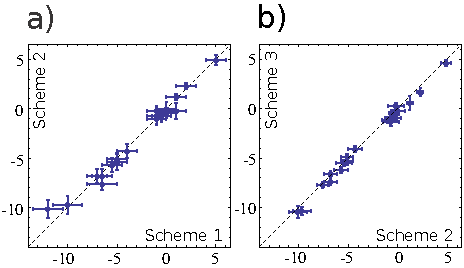
\includegraphics[width=\columnwidth]{Fig5}
    \caption{
    Correlation plot of \gtwoCH{} values with corresponding errors (see Table \ref{tab:gtwo}) obtained with the aid of Schemes 1-3. A reference set of 20 methylene groups characterized by a good signal to noise ratio and the absence of signal overlap was used. The set includes various types of methylene groups spaced differently from the backbone and covering the entire typical range of values.}
    \label{fig:cp}
\end{figure}

\subsection{Scheme 2: \oneJch-modulated carbon-detected experiment}
\label{subseq:scheme2}

\begin{figure*}
  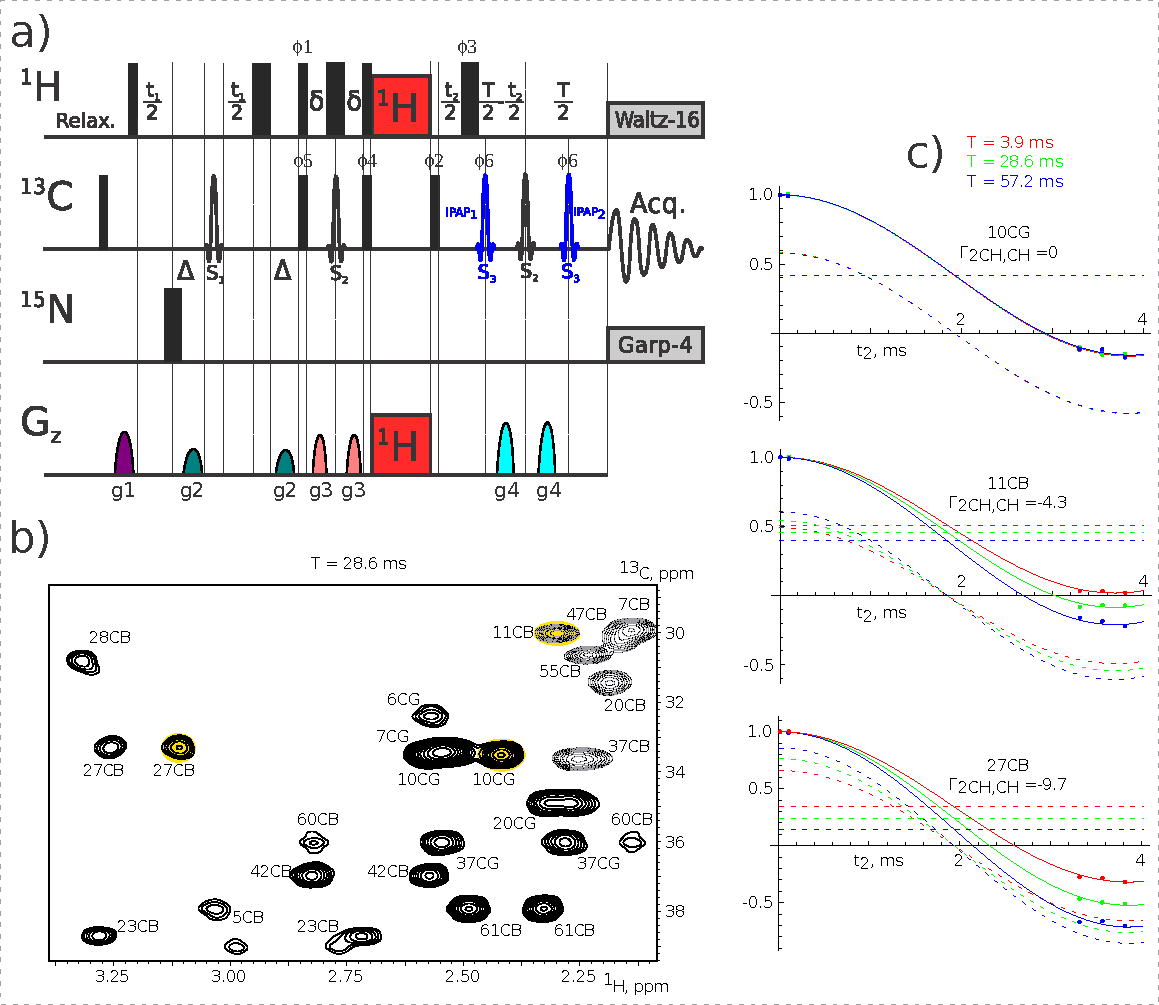
\includegraphics[width=1.0\textwidth]{Fig2}
  \caption{
  a) The pulse sequence of a 2D \hlab-\clab{} carbon-detected 
  \oneJch-modulated experiment (Scheme \ref{subseq:scheme2}) to measure 
  \gtwoCH. 
  Narrow and thick bars represent 90\degree{} and 180\degree{} pulses.
  Semi-constant-time \hlab{} States-{TPPI} sampling is implemented 
  with the aid of $t_1$ delay and $\varphi_1$; 
  {INEPT} delays are $\Delta = 2\delta = 1/(4 \oneJch)$; 
  transverse relaxation delays $T$ are 3.9, 28.6 and 57.2 ms; 
  $t_2$ delay is used for \oneJch{} evolution. 
  The red box represents the same block as in Fig. \ref{fig:scheme1}. 
  \nlab- and \hlab-decoupling are applied during acquisition. 
  S1 is a $500 \mu s$ long \clab{} inversion adiabatic Chirp pulse. 
  S2 is a $220 \mu s$ long 180\degree{} Q3 pulse (the offset at 36 ppm). 
  S3 (a $265 \mu s$ long inversion IBurp1 pulse with the offset at 145 ppm) 
  are applied for virtual {IPAP} decoupling by simultaneous altering the 
  {IPAP1} ($T/4$ or 4.5 ms) and {IPAP2} ($T/4$ or 0 ms) delays. 
  Gradient pulses with squared sine shape and 1 ms length except for g3 
  (0.6 ms) are used. The g1-g4 gradient strengths are as follows: 
  27\%, 37\%, 47\%, 57\% whereas 100\% corresponds to 53.5 G/cm. 
  The default phase is $x$ and the phase cycle is: 
  $\varphi_1 = y, -y$; 
  $\varphi_2 = 2(x), 2(-x)$; 
  $\varphi_3 = 4(x), 4(-x)$; 
  $\varphi_4 = 8(x), 8(-x)$; 
  $\varphi_5 = 16(y), 16(-y)$; 
  $\varphi_6 = 32(x), 32(-x)$; 
  $\varphi_\text{REC} = 2[2(x, -x, -x, x), 4(-x, x, x, -x), 2(x, -x, -x, x)]$. 
  b) A fragment of the 2D \hlab-\clab{} \oneJch-modulated 
  carbon-detected   spectrum, obtained at $T = 28.6$ ms and 
  $t_2 = 8\,\mu s$. 
  Approximation of the signal intensities as a function of $t_2 = 0.008$, 
  0.1, 3.3, 3.55, 3.8 ms is shown on the (c) panel
  }
  \label{fig:scheme2}
\end{figure*}

Explicit observation of methylene triplets in the carbon-detected experiment 
though allow directly obtaining \gtwo{} from the ratios of triplet intensity 
has two distinct disadvantages: low sensitivity as a result of signal splitting and considerable overlap of triplets. 
In order to enhance sensitivity and increase resolution, we replace the 
\oneJch-resolved approach (Fig.~\ref{fig:scheme1}b) by the \oneJch-modulated 
one (Fig.~\ref{fig:scheme2}b), 
effectively converting triplets in the \clab{} direction to singlets 
(Scheme 2). The \oneJch-modulated constant-time {HSQC}-based proton-detected 
method has been sugges\-ted earlier for methyl groups \cite{zhang_probing_2006,lesovoy_nmr_2017}.
However, in the case of methylene groups back {INEPT} can transfer only the 
sum of the \qouter{} components \TermOuter{} of the \clab{} triplet for 
\hlab{} acquisition, whereas the \qinner{} component \TermInner{} does not 
evolve under \oneJch{} scalar coupling Hamiltonian, and hence cannot be 
transferred to \hlab{} nuclei for detection. Therefore, the intensity of a methylene signals approximated by the expression $I_{out} \cos (2 \pi \cdot \oneJch \cdot t_2) $ can provide only \oneJch{} constants. We used their values as input for 
further analysis. In order to achieve simultaneous detection of the 
\qinner{} and \qouter{} components of the \clab{} triplet, we suggest a 
carbon-detected modification of the experiment of Zhang et al. 
\cite{zhang_probing_2006}, as illustrated by Fig.~\ref{fig:scheme2}a. 
In the experiment under consideration, as opposed to the one illustrated 
by Fig.~\ref{fig:scheme1}a, an inversion 180\degree{} proton pulse 
$\varphi_3$ is added during the transverse relaxation delay $T$ to 
refocus the effect of \oneJch{} couplings. These arrangements allow 
obtaining carbon singlets, which can be narrowed via pure 
shift techniques, see Fig.~\ref{fig:scheme2}b. 

The dependence of the singlet intensity upon $t_2$ can be approximated by the 
equation
\begin{equation}
  \label{eq:sch2:time}
  I(t_2) = \Iinn + \Iout \cos (2\pi \cdot \oneJch \cdot t_2 ) 
\end{equation}
at fixed values of \oneJch{} coupling constants determined earlier. 
Fig.~\ref{fig:scheme2}c illustrates such an approximation for the same 
groups as in Fig.~\ref{fig:scheme1}c. 
It is worth noting that since the \oneJch{} are fixed, it is reasonable to 
set the values of $t_2$ delay at $1/(2 \cdot \oneJch)$ and zero, which approximately 
corresponds to the sum $\Iinn + \Iout$ and the difference 
$\Iinn - \Iout$, respectively. Thus, the dependence of the $\Iout / \Iinn$ 
upon $T$ can be approximated by the equation 
\begin{equation}
  \label{eq:sch2:intensity}
  T \cdot 2 \gtwo + A = -ln \biggl(\frac{\Iout}{\Iinn} \biggr) 
\end{equation}
in line with earlier works \cite{zhang_probing_2006,carlomagno_errors_2000}. 
We compared this scheme to the one illustrated by Fig. \ref{fig:scheme1}. 
The results are 
summarized in Fig.~\ref{fig:cp}a and indicative of lower random errors 
in the latter case, without systematic discrepancies between the methods. 

\subsection{Scheme 3: \oneJch-modulated proton-detected experiment}
\label{subseq:scheme3}

\begin{figure*}
  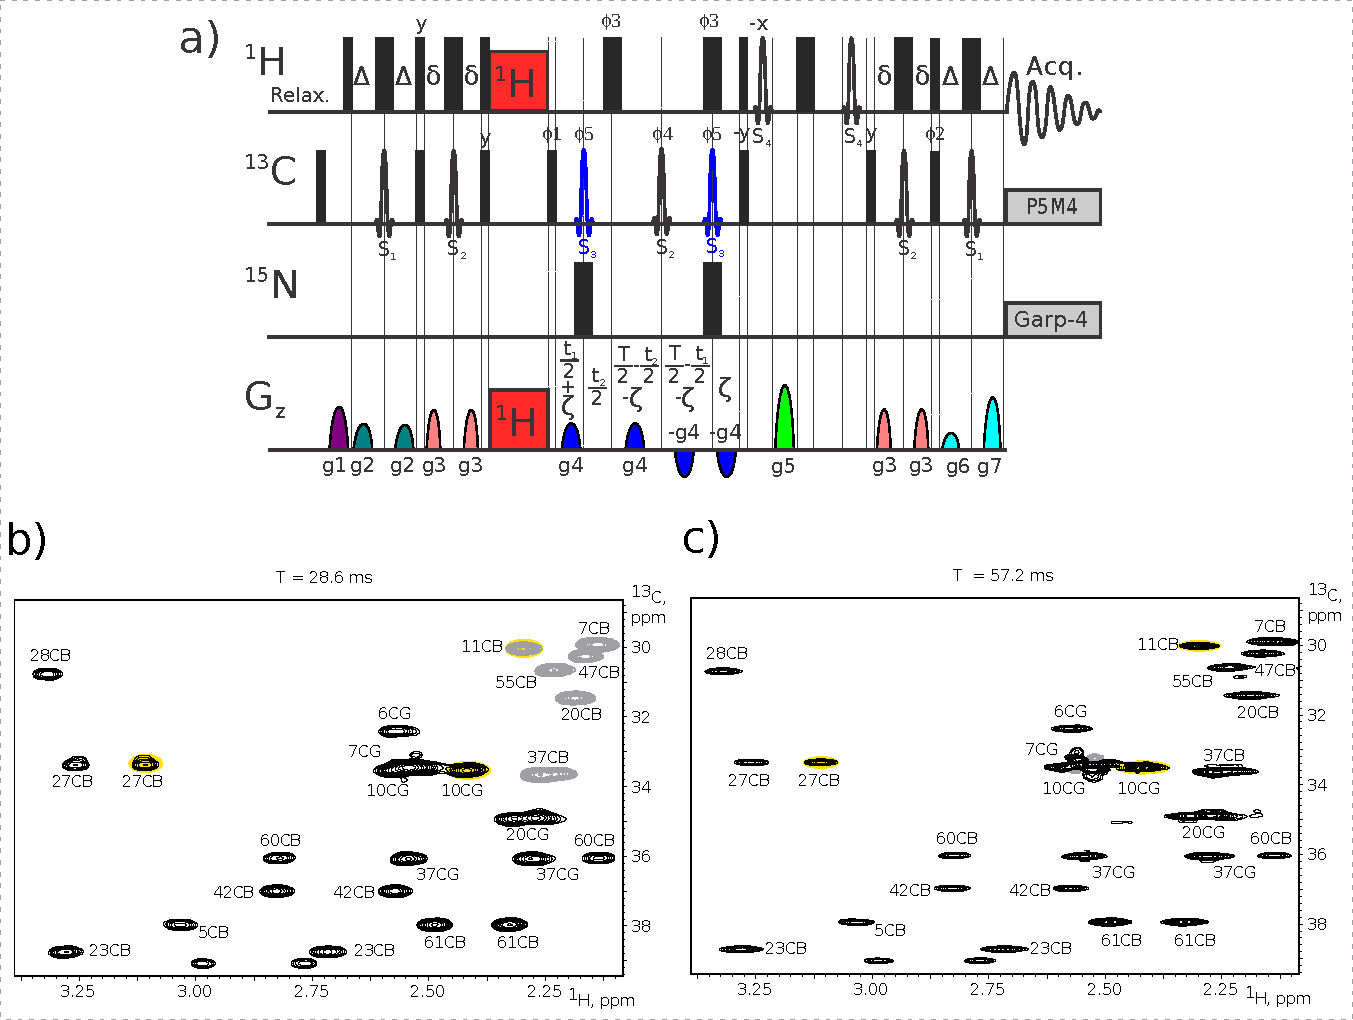
\includegraphics[width=1.0\textwidth]{Fig3}
  \caption{
    a) The pulse sequence of a 2D \hlab-\clab{} proton-detected 
    \oneJch-modulated experiment (Scheme \ref{subseq:scheme3}) 
    to measure \gtwoCH. Narrow and thick bars represent 90\degree{} 
    and 180\degree{} pulses. Constant-time \clab{} Echo-Antiecho 
    sampling is implemented with the aid of $t_1$ delay and g4; 
    INEPT delays are $\Delta = 2\delta = 1/(4 \oneJch)$; 
    transverse relaxation delays $T$ are 28.6 and 57.2 ms; 
    $t_2$ delay is used for \oneJch{} evolution; $\zeta = 1.2$ ms 
    delay appears only for g4. The red box represents the same block 
    as in Fig. \ref{fig:scheme1}. \nlab- and \clab-decoupling are applied 
    during acquisition. 
    S1 is a $500 \mu s$ long \clab{} inversion adiabatic Chirp pulse. 
    S2 is a $220 \mu s$ long 180\degree{} Q3 pulse (the offset at 36 ppm). 
    S3 is a $265 \mu s$ long inversion IBurp1 pulse (the offset at 145 ppm).
    S4 is a 90\degree{} sinc-shaped water-selective \hlab{} flip-back pulse with a duration of 3 ms.
    Gradient pulses with squared sine shape and 1 ms length except for g3 
    (0.6 ms) are used. The g1-g7 gradient strengths are as follows: 
    27\%, 37\%, 47\%, 40\%, 57\%, 10\%, 50.2\% whereas 100\% corresponds to 53.5 G/cm. Continuous wave water presaturation at 0.04 mW was used during the relaxation delay for better suppression.
    The default phase is $x$ and the phase cycle is: 
    $\varphi_1 = y, -y$; 
    $\varphi_2 = 2(x), 2(-x)$; 
    $\varphi_3 = 4(x), 4(-x)$; 
    $\varphi_4 = 8(x), 8(-x)$; 
    $\varphi_5 = 16(x), 16(-x)$; 
    $\varphi_\text{REC} = 8(x, -x, -x, x)$. 
    For each successive $t_1$ value, $\varphi_1$ and the phase of the receiver are incremented by 180\degree. 
    b, c) A fragments of the 2D \hlab-\clab{} \oneJch-modulated proton-detected spectra obtained at $T = 28.6$, 57.2 ms and $t_2 = 8 \mu s$, 
    respectively.
  }
  \label{fig:scheme3}
\end{figure*}

Despite the improved resolution in the \clab{} spectrum, the Scheme 2 
illustrated by Fig.~\ref{fig:scheme2} has several weaknesses: low 
sensitivity during 
\clab{} acquisition, peak bro\-ade\-ning due to \oneJcc{} couplings, and 
cross-correlation effects during \clab{} acquisition, resulting in 
$A \ne 0$ in equations \eqref{eq:sch1:intensity} and \eqref{eq:sch2:intensity} 
at the data processing stage. 
To eliminate these weaknesses, 
we designed Scheme 3: a \oneJch-modulated proton-de\-tec\-ted experiment 
(see Fig.~\ref{fig:scheme3}). This constant-time {HSQC}-based method 
transfers only the sum 
of the \qouter{} components \TermOuter{} for detection via back refocused 
{INEPT}, but we cannot transfer the central component in this way. However, 
we can adjust all the components in advance, so that the resultant 
composition is made up of the two \qouter{} components and the \qinner{} one with the intensity ratio 1:2:1. 
To make the adjustment we can suppress all \hlab{} containing terms 
(see equations \eqref{eq:sigmainout})
between points \enquote{a} and \enquote{b} of the pulse sequence (Fig. \ref{fig:scheme3}a) 
applying the $90\degree$ proton pulse followed by a gradient. 
At the point \enquote{a} there are two key spin states that should be considered: the target 
$C_x$ coherence and the unwanted $C_x H_z H'_z$ term that should
be eliminated from the back INEPT transfer and the acquisition. The block between points 
\enquote{a} and \enquote{b} keeps $C_x$ untouched and converts $C_x H_z H'_z$ 
to a zero-quantum state 
$C_x \text{ZQ}_x =  C_x (H_x H'_x + H_y H'_y)$.
The $ZQ_x$ state evolves during the \enquote{a}--\enquote{b} delay with the frequency
$\Omega_{ZQ}=\omega_{H}-\omega_{H'}$ under the chemical shift Hamiltonian
(equations [2.258] and [2.259] in 
\cite{cavanagh_protein_2007}), and
this evolution is refocused by the 180\degree{} \hlab-pulse at the middle of the 
\enquote{a}--\enquote{b} time period:
\begin{align}
  \label{eq:zqx:refocus}
  \overset{\text{\enquote{a}}}{ZQ_x}  
    \xrightarrow{t} & ZQ_x \cos \Omega_{ZQ}t + ZQ_y \sin \Omega_{ZQ}t
    \xrightarrow{} \nonumber \\
    \xrightarrow{\text{180\degree (\hlab)}} & 
      ZQ_x \cos \Omega_{ZQ}t - ZQ_y \sin \Omega_{ZQ}t
      \xrightarrow{t} \overset{\text{"b"}}{ZQ_x}
\end{align}
where $ZQ_y = H_y H'_x - H_x H'_y$. 
After the time point \enquote{b} the $C_x ZQ_x$ coherence evolves to undetectable 
terms during the refocused 
back INEPT transfer, while the absent $ZQ_y$-containing terms would be transformed 
to an anti-phase coherence 
disturbing signal shapes. During the last back INEPT transfer, the evolution of the target coherence is:
\begin{align}
\label{eq:term3:target}
   \overset{\text{\enquote{b}}}{C_x} & \xrightarrow{\text{back INEPT}} 
   \overset{\text{Receiver}}{H_x + H'_x}
\end{align}    
resulted in pure absorption in-phase observable signals as expected. All  
 multispin density operators which contain $ZQ_x$ are converted to undetectable terms at the beginning of the acquisition time:
\begin{subequations}
\label{eq:backZQx}
\begin{align}
   \label{eq:term3:zqx}
   \overset{\text{\enquote{b}}}{ZQ_x} & 
     \xrightarrow{\text{back INEPT}} 
     \overset{\text{Receiver}}{ H_y H'_y +  H_z H'_z} \\
   \label{eq:term3:cxzqx}
   {C_x ZQ_x} & \xrightarrow{\hphantom{\text{back INEPT}}} -\tfrac{1}{2}C_x + 2 C_x H_x H'_x \\
   \label{eq:term3:cyzqx}
   {C_y ZQ_x} & \xrightarrow{\hphantom{\text{back INEPT}}} C_z (H_y H'_y + H_z H'_z)
\end{align}
\end{subequations}
But $ZQ_y$ proton modes (if any in point \enquote{b}) would be converted to some detectable antiphase dispersive terms:

\begin{subequations}
\label{eq:backZQy}
\begin{align}
   \label{eq:term3:zqy}
     \overset{\text{\enquote{b}}}{ZQ_y} & \xrightarrow{\text{back INEPT}}
     \overset{\text{Receiver}}{C_z (H_z H'_y -  H_y H'_z )} \\
   \label{eq:term3:cxzqy}
   {C_x ZQ_y} & \xrightarrow{\hphantom{\text{back INEPT}}} \tfrac{1}{2}C_y ( H'_x- H_x ) \\
   \label{eq:term3:cyzqy}
   {C_y ZQ_y} & \xrightarrow{\hphantom{\text{back INEPT}}} \tfrac{1}{2}( H_z H'_y-  H_y H'_z )
\end{align}
\end{subequations}
As a result, the suggested scheme of 
ZQ evolution allows making accurate and precise measurements of 
\gtwoCH{} with all the advantages of proton detection in the absence 
of \clab{} triplets. 

The product operator formalism of $ZQ_{x,y}$ evolution described above is not appropriate when the 
chemical shift difference between methylene protons is of the same order as ${^2\!J_{\text{HH}'}}$ 
coupling constant \cite{cavanagh_protein_2007,benesi_primer_2015}. Scheme~2 above or the scheme in Fig.~\ref{fig:scheme4} may be more suitable for such cases.
A solution to this problem (at the expense of signal to noise ratio) could also be the increasing of $ZQ_x \rightarrow{} ZQ_y$
refocusing delay (\enquote{a} -- \enquote{b} in Fig. \ref{fig:scheme3}) to guarantee
complete relaxation of proton coherences.

The intensity of a signal in the experiment represented in 
Fig.~\ref{fig:scheme3} can be approximated by the same expression 
\eqref{eq:sch2:time} as for Scheme 2.
Analysis of the time evolution yields the ratio $\Iout/\Iinn$, then \gtwoCH{} can be found from the 
equation:
\begin{equation}
\label{eq:sch3:intensity}
 2 \gtwo \cdot T = -ln \biggl(\frac{\Iout}{\Iinn} \biggr) 
\end{equation}
As opposed to the experiment shown in Fig.~\ref{fig:scheme2}, 
the step-wise increase of 
$T = N/(2 \oneJcc) = N \cdot 14.3$ ms results in the enhancement of resolution 
in the \clab{} dimension in the third experiment (see 
Fig.~\ref{fig:scheme3}b,c). 
For \labNHtwo{} groups, the direct \nlab{} analogue of the pulse sequence
from the Fig.~\ref{fig:scheme3} could similarly provide the $\Iinn/\Iout$ ratio. 

Comparison of the Schemes 1-3 described above is summarized in
Fig.~\ref{fig:cp}b and indicative of the improved accuracy of the third 
method without systematic deviation from the reference carbon-detected
approaches.

\subsection{Applying \oneJch-modulation for measurement of \gtwo{}}
\label{subseq:gtwoblock}

The concept of \oneJch-mo\-du\-la\-ted approach applied in sections
\ref{subseq:scheme2} and \ref{subseq:scheme3} is useful to develop numerous pulse sequences for measurement of \gtwoCH{}.

The first, sophisticated $\hlab \rightarrow{} \clab$ INEPT magnetization 
transfer followed by {ZQC} suppression block has been motivated by the gain in sensitivity. We also developed and tested less 
sensitive schemes which started from 90\degree{} \clab{} pulse only (data not shown) or from \hlab--\clab \{NOE\} signal enhancement by \hlab{} irradiation (illustrated in Fig.~\ref{fig:scheme5}). Both schemes avoids the arising of {ZQC} before \gtwo{} relaxation delay without any observable difference.

The second transfer of the target $C_z$ magnetization to \oneJch-coupled
protons for detection is not the only viable
option. $C_z$ magnetization can be transferred employing 
3D {(H)CC(CO)NH} {TOCSY} sche\-me as in \cite{zheng_measurement_2004}, \oneJch-modulated version of this experiment is illustrated in Fig. \ref{fig:scheme4}.
Other ways of $C_z$ magnetization transfer may include  CBCA(CO)NH
experiment \cite{yang_1h13c_1999,yang_study_1998} or {INEPT}
to $C_\alpha H_\alpha$ \cite{banci_side_2001}. These
alternative options of detection are associated with some advantages and
drawbacks: offering better resolution, they compromise sensitivity and
become dependent on the remoteness of the methylene groups from the
backbone. 

\section{Discussion}
Methylene groups are present in 17 out of 20 proteinogenic amino acids
(Table \ref{tab:gtwostats}), and hence their relaxation parameters provide a detailed
snapshot of the dynamics of any protein. Herein, we suggest an accurate 
and precise methods of measurement of the dipole/dipole transverse
cross-correlatied relaxation rate \gtwo{} of me\-thy\-le\-nes and primary 
amines with 
the use of the \oneJch-modulated approach (Schemes 2 and 3). These 
experiments allowed us to resolve signals and
quantify \gtwoCH{} parameters for 89 out of 90 methylenes 
(see Table \ref{tab:gtwostats} and Fig.~\ref{fig:g2:struct}A) 
in the uniformly \nclab{} labelled {NTII} with random errors ranging 
from $~0.3$ to $~0.7$ $s^{-1}$ in the typical band of measured parameters 
from $-10$ to $5$ $s^{-1}$. The approach differs considerably from the ones
published earlier \cite{banci_side_2001,zheng_measurement_2004}, and has
some advantages allowing us to recommend it as a method of choice for
quantification of \gtwoCH{} and \gtwoNH{} in a broad spectrum of 
uniformly \nclab{} labelled proteins.

Prior attempts to quantitatively measure methylene \gtwoCH{} 
\cite{banci_side_2001,zheng_measurement_2004} explicitly detected
\oneJch-resolved triplets on another nucleus ($C_\alpha H_\alpha$ or NH) 
and then analysed the ratio of intensities of the triplet components.
Such an approach compromises sensitivity for two reasons: first, due 
to the splitting of a singlet into a triplet; and second, due to 
attenuation of a signal during transfer of the term onto the 
auxiliary remote nucleus. This least-evil solution is specific to 
methylene as a spin system since the central component of the carbon 
triplet \eqref{eq:sigmainner} cannot be transferred to methylene 
protons \cite{zhang_probing_2006} in order to take
advantage of high sensitivity. For similar reasons, \oneJch-modulated
approach offering enhanced resolution and sensitivity cannot be used
directly. As opposed to the case of methylenes, two standard approaches 
to sensitivity and resolution enhancement, {INEPT} and 
\oneJch-modulated experiment, have been successfully implemented for 
methyls \cite{zhang_probing_2006,lesovoy_nmr_2017}. 

The accurate and sensitive measurement of \gtwoCH{} in \CHtwo{} groups
is achieved in Schemes~2 and 3 as the combination of well-known NMR
techniques described previously. The novelty of Scheme~3 consists in the specific
combination of three elements: (1) the intensity adjustment of 1:2:1 carbon triplet is
applied twice, before and after relaxation delay 
(the adjustment before relaxation delay was routinely used in all previous schemes
\cite{banci_side_2001,zheng_measurement_2004,yang_study_1998}; 
(2) the \oneJch-modulation is used for methylenes
(measuring \gtwoCH{} in methylenes 
without the second intensity adjustment is useless \cite{yang_probing_2011});
(3) a zero-quantum coherence is converted to separate undetectable terms (the second intensity adjustment inevitably produces a zero-quantum 
coherence which evolves under the chemical shift Hamiltonian 
$ZQ_x\xrightarrow{} ZQ_y$ and would disturb signal shape and intensity without special attention to its evolution).

Let us analyze random and systematic errors contributing to the measured
values of methylene \gtwoCH{} based on guidelines 
from the work of Carlomagno and Griesinger \cite{carlomagno_errors_2000}. 
For this purpose, we shall compare the three 
tested pulse sequences from the viewpoint of selection of the most 
suitable one for a protein of a particular category, optimization of
experimental parameters and uncertainty sources.

According to \cite{carlomagno_errors_2000}, constant time delay 
$T = \allowbreak N/\allowbreak (2\cdot~\oneJcc) \allowbreak = N\cdot 14.3$ ms should approximately scale as 
$1/R_2$ for the case of  $\gtwoCH$ subjected to the condition: 
$\gtwoCH\cdot T < 1$. The direct measurement of $R_2$ is unavailable 
for methylenes, since the \clab{} transverse relaxation decay is 
multiexponential as a result of cross-correlation
effects \cite{yang_probing_2011}, as well as the influence of $R_{ex}$ in the absence of {CPMG}. Nevertheless, a guess for the integer  $N$ allowing the proper scaling of $T$ can be made from the constant-time \clab{} {HSQC} experiment.

\begin{figure}
    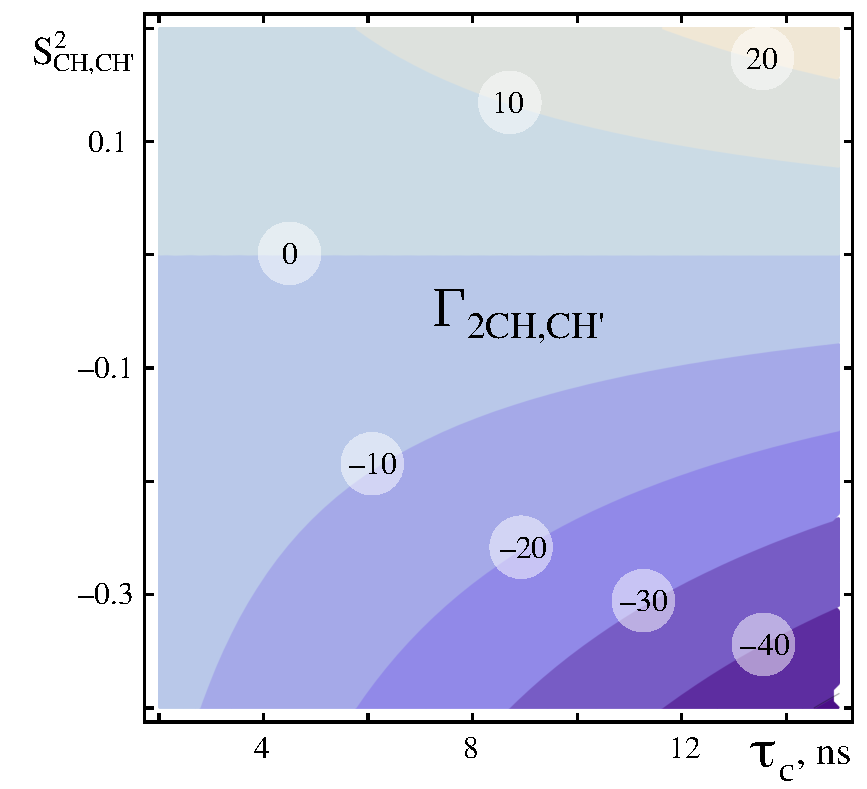
\includegraphics[width=\columnwidth]{Fig4}
    \caption{
    Contour plot of 
    \gtwoCH{} as a function of the overall correlation time $ \tau_c $ 
    and the cross-correlation order parameter \StwoCHp{}. Relaxation rates 
    were calculated from eq. \eqref{eq:gtwo:tauc} at $\omega_\text{H}/2 \pi = 800\,\text{MHz}$.
    \label{fig:g2contours}Assuming tetrahedral bond angle in \CHtwo{} group completely restricted motion (rigid molecule) corresponds to $\StwoCHp{}=-1/3$; cross-correlation order parameter $\StwoCHp{}=1/9$ matches the case of entirely free rotation.
    }
\end{figure}

As stated in \cite{carlomagno_errors_2000}, processing experimental data with different $T$ may require the use of $f(T) = A + \gtwoCH\cdot T$ with $A \ne 0$ for approximation. A possible reason for that is a distortion of a methylene \clab{} triplet signal 
at the stage of detection. This issue equally applies to both
carbon-detected experiments discussed in the present work, whereas proton-detected experiments are the 
least affected by the need to use $A \ne 0$ since it detects 
transferred terms proportional to the sum of \qinner{} and 
\qouter{} components of the triplet.

It's noteworthy that the dependence of \gtwoCH{} 
as a function of the overall correlation time $ \tau_c $ of a molecule  demonstrates the growth of the \gtwoCH{} absolute 
value with the increase of  $ \tau_c $
(Fig.~\ref{fig:g2contours}). This  consideration allows
minimizing $N$ in the experiment without the increase of the resulting \gtwoCH{} 
relative error for slowly tumbling proteins. Furthermore, in contrast to \clab{} $R_1$ and heteronuclear NOE, the measurement of \gtwoCH{} do not suffer 
from systematic errors caused by \clab{}$-$\clab{} auto- and cross-relaxation regardless of $ \tau_c $
\cite{yang_probing_2011,jin_cross-correlation_2003}.

While talking about the systematic errors of the analysis, it should be
mentioned that the \qinner{} component 
$\Iinn{} = 2I(0)\exp \bigl( -{\gtwo \cdot T\bigr)}$ \eqref{eq:gint:abba} 
is not affected by CSA\slash dipole cross-cor\-re\-la\-tion \gtwoCSA{} 
at all. The effects of \gtwoCSA{} to the \qouter{} components are negligible as follows from the next considerations. 
In contrast to the backbone NH groups and aromatic CH groups, 
the aliphatic carbons exhibit relatively small values of CSA 
\cite{ferrage_chapter_2017,banci_side_2001,zheng_measurement_2004};
therefore, $\gtwo$ is dominated over $\gtwoCSA$
in the sum of the \qouter{} components \eqref{eq:gintensity}: 
\begin{multline}
    \label{eq:neglectCSA}
    \Iout(T) = \Ioutone(T) + \Iouttwo(T) = \\
      = I(0)\Bigl[\exp\bigl({-(\gtwo + 2\gtwoCSA) \cdot T}\bigr) + \\  
       + \exp\bigl({-(\gtwo - 2\gtwoCSA) \cdot T} \bigr) \Bigr]= \\
     = 2I(0)\exp\bigl({-\gtwo \cdot T} \bigr) 
             \bigl(1+
               \underbrace{ 2(\gtwoCSA \cdot T)^2+\cdots}_{\text{Small,}\ll 1}
            \bigr) 
      \approx \\
      \approx 2I(0)\exp \bigl( {-\gtwo \cdot T} \bigr)
\end{multline}

We evaluated the contribution of $2(\gtwoCSA \cdot T)^2$ 
 from the \qouter{} components using equation \eqref{eq:gcsafromint} and
 experimental data obtained for Scheme~1.
 A maximal value of $2(\gtwoCSA \cdot T)^2$ obtained for 20 well resolved triplets in Scheme~1 turned out to be less
 than 0.03. Furthermore, the same value was estimated
 from those publications where an explicit \clab{} triplet structure 
 is visible  on the published representative NMR slices, namely, 
 figure~5a in \cite{yang_study_1998}, 
 figure~1 in \cite{yang_1h13c_1999}, 
 figure~3 in \cite{banci_side_2001} and 
 figure~3 in  \cite{zheng_measurement_2004}. All the figures
 support $2(\gtwoCSA \cdot T)^2 \ll 1$ for most proteins and 
 typically used transverse relaxation delays $T$.

It is noteworthy that only the third scheme (out of the three suggested 
in this work) is applicable for determining the ratio
\begin{equation}
    \label{eq:cnst1}
    C_1 = \frac{\Iinn}{\Ioutone + \Iouttwo}
\end{equation}
of side chain \NHtwo{} groups. Since the effects of \gtwoNNH{}
are not negligible, in order to obtain the \gtwoNH{} values 
(see BMRB 19704), the ratio
\begin{equation}
    \label{eq:cnst2}
    C_2 = \frac{\Ioutone}{\Iouttwo}
\end{equation}
has to be additionally measured with the aid of conventional 2D 
\hlab-\nlab{} constant-time {HSQC} experiment without the 180\degree{} 
proton pulse responsible for refocusing of \oneJnh{} evolution, 
and thus resulting in doublets in \nlab{} direction. In this case 
(see Table 
\ref{tab:gtwo}), \gtwoNH{} values can be calculated from equations \eqref{eq:cnst1}, \eqref{eq:cnst2} as
\begin{multline}
    \label{eq:gtwoNH2}
    4\gtwoNH\cdot T = 
    -\ln \biggl( \frac{4 \Ioutone\Iouttwo}{\Iinn^2} \biggr)= \\
    = -\ln \biggl( \frac{4 C_2}{C_1^2 (1+C_2)^2} \biggr)
\end{multline}

In the first two carbon-detected experiments the accuracy of \gtwoCH{} determination and the fraction of resolvable signals can be substantially increased employing pure shift methods in the direct \clab{} dimension: \oneJcc-decon\-volution processing \cite{shimba_elimination_2003,kazimierczuk_non-uniform_2015} as well as band-selective or spin-state-selective decoupling \cite{zangger_pure_2015}. Nevertheless, the first carbon-detected experiment (Scheme~1) mostly serves as a reference approach, whereas \oneJch-modulated schemes are recommended for direct applications. It should be noted, that since the analysis of the second and the third \oneJch-modulated 
experiments involves the values of $\cos(2\pi J t_2)$  at 
$2\pi J t_2 = 0$ and $\approx \pi$ an insignificant 
spread of the \oneJch{} values caused by the different environment of 
identical amino acid residues would, for all practical purposes, not 
affect the results of approximation. Hence, 27 different averaged 
values of \oneJch{} can be used at corresponding \CHtwo{} positions in 
proteins (see Table \ref{tab:oneJch} with 24 \oneJch{} value stacking 
from the data for 
{NTII}), and the value of $\oneJnh{} = -90.4$ Hz can be used at \NHtwo{} 
positions. Supplemental figure \ref{fig:scheme4} include a modification 
(based on 3D {CC(CO)NH} 
{TOCSY}) of the third \oneJch-modulated experiment, having the highest 
resolution, but suffering from the dependence of sensitivity upon the 
spacing between a methylene group and a backbone and upon the 
characteristics of the {NH} signal itself. This 3D experiment requires 
larger storage time, which, however, can be decreased with the aid of 
non-linear sampling methods \cite{kazimierczuk_non-uniform_2015}
that are especially effective in the case of constant-time sampling in 
two \clab{} and \nlab{} indirect dimensions. This modification can be, 
in some cases, optimal for IDP proteins exhibiting low values of 
chemical shift dispersion and transverse relaxation. 

\begin{figure*}
    \centering
    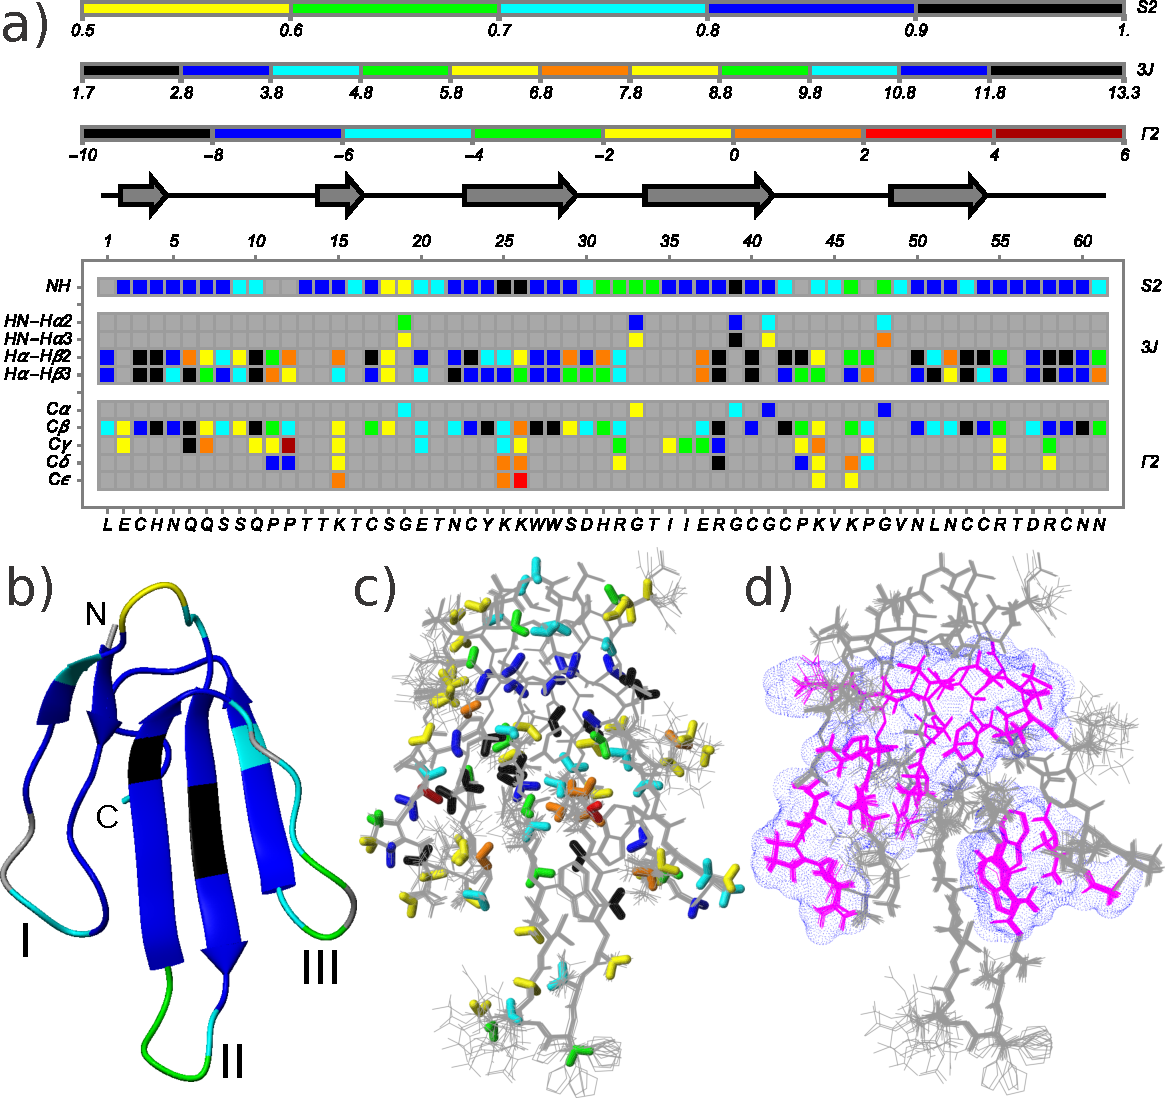
\includegraphics[width=\textwidth]{Fig6}
    \caption{NMR parameters depict NTII flexibility.
    (A) Methylene relaxation parameters \gtwo{} (lower panel) together with
    $^3J_\text{HH}$
    coupling constants (in the middle) and backbone NH order parameters 
    (upper panel) arranged along the sequence of NTII. 
    Color schemes for different data types are shown above the secondary 
    structure diagram. Dark colors (black and blue) correspond to more 
    spatially restricted motions for all data types. 
    In the case of $^3J_\text{HH}$ couplings both constants should be shown dark 
    to reflect totally hindered rotation about N-$\text{C}_\alpha$ or 
    $\text{C}_\alpha$-$\text{C}_\beta$ bonds.
    (B) Ribbon diagram of NTII structure with color coded backbone NH order parameters, the color scheme is the same as on the panel A. 
    Three \enquote{fingers} of the toxin molecule are indicated by Roman numerals.
    (C) \gtwo{} data for methylenes superimposed on the NTII NMR ensemble of 
    spatial structures (20 structures from PDB are drawn by grey lines). 
    Methylenes of the 1-st nmr structure are represented by thick painted 
    sticks  (the color code is the same as on panel A) 
    (D). A generalization of the illustration (C) showing two clusters 
    of methylenes with spatially restricted motions. Residues having 
    at least one methylene with substantially lowered  \gtwo{} values 
    (coded blue or black) are drawn by magenta lines. Accessible surfaces 
    of these residues (blue clouds) merge together to form two clusters. 
    A single exception is G39 which is deeply buried within the big cluster, 
    but coded cyan ($\gtwo=-5.56\,s^{-1}$). 
    }
    \label{fig:g2:struct}
\end{figure*}


\gtwoCH{} in combination with other relaxation parameters (e.g. $R_1$ 
and NOE) can be used both for direct mapping of spectral density functions
\cite{kaderavek_spectral_2016}  and for various interpretations 
giving spatial (order parameters) and temporal (rotational correlation 
times) parameters of internal motions within a \CHtwo{} group.

We should emphasize that $R_1$ and NOE of methylene groups are associated with \emph{auto}{-}cor\-re\-la\-tion order parameter \StwoCH{}, while  \gtwoCH{} is characterized by \emph{cross}-correlation order parameter \StwoCHp{}.
These two parameters are interrelated, e.g. fully restricted motion of a \CHtwo{} group (rigid methylene) results in $\StwoCH=1$ and $\StwoCHp=-1/3$, free unrestricted rotation of a \CHtwo{} group is described by $\StwoCH=0$ and $\StwoCHp=1/9$. 
Different relationships between these order parameters define various motional models discussed by Daragan, Mayo and coworkers  \cite{idiyatullin_simple_2004,daragan_motional_1997,daragan_using_1995}.
One may 
start from simplest models with isotropic overall tumbling of the 
protein and a single axis internal rotation within a \CHtwo{} group (see 
\cite{daragan_motional_1997,zheng_measurement_2004,daragan_using_1995}), 
or continue with more complex multiparametric models
\cite{paquin_multiple-timescale_2008,ferrage_chapter_2017,ghalebani_nmr_2008,kaderavek_spectral_2016} 
requiring the measurement of relaxation parameters at different values 
of magnetic field strength. The need to invoke motional models complicates the interpretation and requires additional measurements, on the other hand, unique information about the local anisotropy of rotation within a methylene group can be gained. Beyond that, \gtwoCH{} (together with other
relaxation parameters) can serve as an experimental reference for
comparison with corresponding parameters calculated from MD
trajectories (see \cite{aliev_motional_2014}).

Methylene relaxation parameters \gtwoCH{} may admit a simple
interpretation related them linearly to cross-correlation order parameters
(see Theory, eq. \eqref{eq:gtwo:tauc}), which strongly depends upon motional restrictions (see discussions about motional restriction maps in the works of Daragan, Mayo and coworkers  \cite{idiyatullin_simple_2004,daragan_motional_1997,daragan_using_1995}). 
Highly restricted motions results in low negative values of \gtwoCH{} and \StwoCHp{}, but (strictly speaking) the converse does not hold. Non-monotonic dependence between the cross- (or auto-) correlation order parameter and the motional amplitude may lead to an ambiguous interpretation of order parameters, e.g. in the case of two state rotational jumps and some other models \cite{daragan_using_1995,idiyatullin_simple_2004}. Positive values of \gtwoCH{} are generally associated with less restricted motion of a flexible ($\StwoCH<0.5$) methylene group. In the following simplified analysis of \gtwoCH{} parameters we will assume: 1) isotropic overall tumbling of the protein, 2) a single axis rotation within a methylene group, 3) a correlation between the value of \gtwoCH{} and the degree of motional restriction within a methylene group.

Interpretation of \gtwoCH{} together with other types of NMR data
may provide additional insights into dynamic features of protein packing.
Specifically, in our study of NTII the most pro\-no\-unce correlation was found between
\gtwoCH{} and $^3\!J_\text{HH}$ coupling constants 
(Fig.~\ref{fig:g2:struct}a), though \gtwoCH{} and backbone NH order
parameters efficiently complement each other. Backbone order parameters 
of NTII give the impression that the protein is extremely rigid 
(Fig.~\ref{fig:g2:struct}a,b). However, side-chain relaxation 
data show surprisingly variable and not always predictable patterns 
of methylene dynamics (Fig.~\ref{fig:g2:struct}a,c). 
For example, Fig.~\ref{fig:g2:struct}a highlight the unusually 
restricted  motions (as supported by $^3\!J_\text{HH}$ values) of R38 side-chain methylenes ($\beta$,$\gamma$, 
and $\delta$). This specific feature of NTII packing can be explained 
by formation of the C-terminal capping motif including the salt bridge between 
the guanidine group of R38 and the C-terminal carboxyl and a dozen of hydrogen bonds, particularly, $61 \allowbreak \text{CO} \allowbreak \cdots 25\text{H}_\zeta$, $61CO_\beta\cdots38H_{H2}$, $60CO_{\delta1}\cdots4H_N$,
$24\-CO\cdots60H_{\delta21}$, $4CO\cdots60H_{\delta22}$ and so on.
It's remarkable that R38 has steric interactions with closely spaced 
side-chains of Q6, H4, N60. These  
residues have very low \gtwoCH{} values (marked by black in Fig.~\ref{fig:g2:struct}a) of $\beta$ and/or 
$\gamma$ methylenes. $^3\!J_\text{HH}$ data support highly restricted motions for H4 and N60, but not for Q6. R38, Q6, H4, and N60 together 
with 5 cysteines (except C17), 3 prolines (not including C17 and P47), and some 
other residues have at least one methylene with low \gtwoCH{} and 
define the big cluster of spatially restricted dynamics (see
Fig.~\ref{fig:g2:struct}, c and d). Another smaller cluster is formed 
around two neighboring tryptophanes and includes also N50 and G48.  $^3\!J_\text{HH}$ data verify spatially restricted dynamics for all side chains of smaller cluster except G48. More sophisticated models (which require additional measurements) may be more appropriate for Q6, G41, and G48.
The specified clusters correlate, but don't agree exactly with the 
hydrophobic core of the molecule. Actually, a significant correlation 
of side-chain order parameters with accessible surface area (ASA) 
has been reported earlier for NH groups of arginines and tryptophanes
\cite{buck_structural_1995}. However, we identified some methylenes 
with low value of \gtwoCH{}, but substantial ASA. And vice versa, 
noticeable amounts of methylenes have relatively high values of 
\gtwoCH{}, but close to zero ASA. Anyway it's intriguing that 
functionally active regions of NTII (receptor- and membrane-binding 
sites) is absolutely free from methylenes with spatially restricted dynamics.

\section{Conclusions}
\label{seq:conclusions}
We suggest an accurate and precise methods of measurement of the dipole/dipole 
transverse cross-correlated relaxation rate \gtwoXH{} of methylenes and primary 
amines for uniformly \nclab-labeled proteins (Schemes 2 and 3). In the search for the 
best approach, we tested three ways to measure \gtwoCH: 2D carbon-detected 
\oneJch-resolved, 2D carbon-detected \oneJch-modulated, and 2D proton-detected
\oneJxh-modulated experiments, with the sequential decrease of signal overlap 
and the enhancement of measurement accuracy (in the order the experiments are 
listed). The latter experiment requires special attention to a zero-quantum coherence evolution; it 
also allows measuring \gtwoNH{} of primary amines (Asn and Gln side chains) 
with the same efficiency despite the low gyromagnetic ratio of \nlab.
Since measurements and analysis of $R_2$ in \XHtwo{} groups run into serious difficulties, \gtwo{} 
effectively provides the only practical opportunity to obtain information about the 
value of the spectral density function at zero frequency $J(0)$ without any 
contribution of $R_\text{ex}$. Our 2D experiments have the sensitivity similar 
to that obtained by constant-time {HSQC}-based methods, but independent 
of the remoteness of the \CHtwo{} group from the backbone and of the 
characteristics of the backbone NH signal. To enhance the accuracy of \gtwoCH{}, 
we used \oneJch{} coupling constants, which could be obtained by the experiment
suggested earlier for the measurement of \gtwoCH{} for methyls 
\cite{zhang_probing_2006}. However, in the case of methylenes, this experiment 
can provide only \oneJch{} values. In addition to that, we modified the 
{(H)CC(CO)NH} {TOCSY} 3D pulse scheme \cite{zheng_measurement_2004}, and the 
updated experiment has gained the increased sensitivity and resolution in 
comparison with the original one. Different pulse schemes for the measurement 
of \gtwoXH{} described in the present work were compared with the intention 
of guiding the optimisation of experimental parameters for various proteins. 
We give an overview of the application of \gtwoCH{} for the extraction of 
dynamic parameters of intramolecular motion within a methylene group. 
Pulse sequences developed in this and our earlier side-chain study \cite{lesovoy_nmr_2017} are available for 
Bruker Avance spectrometers at \url{https://github.com/lesovoydm/NMR-side-chain-relaxation} or \url{http://www.ibch.ru/en/unit/nmr#research}. 


\begin{acknowledgements}
The work was supported by the Russian Science Foundation grant 
\#18-14-00375: pulse sequence development and data analysis.  
{NMR} experiments were carried out using the equipment 
provided by the {IBCH} core facility ({CKP} {IBCH}, grant 
{RFMEFI62117X0018} from Russian Ministry of Education and Science) 
and partially supported by the 
Russian Academy of Science program "Molecular and cellular biology" and the Russian Foundation for Basic Research grant \#18-04-01289. 
The authors thank Dr. A.A.~Shul\-ga for the sample of 
uniformly \nclab-labeled Neurotoxin~II. 
\end{acknowledgements}

% BibTeX users please use one of
%\bibliographystyle{spbasic}      % basic style, author-year citations
%\bibliographystyle{spmpsci}      % mathematics and physical sciences


\bibliographystyle{spphys}       % APS-like style for physics
\bibliography{G2_Method}   % name your BibTeX data base
%\bibliographystyle{plain}
%\printbibliography

% Non-BibTeX users please use
%\begin{thebibliography}{}
%
% and use \bibitem to create references. Consult the Instructions
% for authors for reference list style.
%
%\bibitem{RefJ}
% Format for Journal Reference
%Author, Article title, Journal, Volume, page numbers (year)
% Format for books
%\bibitem{RefB}
%Author, Book title, page numbers. Publisher, place (year)
% etc
%\end{thebibliography}

\end{document}
% end of file template.tex